\documentclass{beamer}

\usepackage{tikz}

% switch off the fancy navigation symbols
\setbeamertemplate{navigation symbols}{}

\title{${}$\\[3.5em]10th International\\
Satisfiability Modulo Theories\\
Competition\\[.7em]
SMT-COMP 2015\\[3em]}

\author{Sylvain Conchon \and David D{\'e}harbe \and Tjark Weber}

\institute{}

\date{}

\logo{\vspace{2.7cm}
\includegraphics[width=\textwidth]{laurels}\hspace{.8cm}}

\newcommand{\record}[1]{\textcolor{red}{#1}}

\begin{document}

%%%%%%%%%%%%%%%%%%%%%%%%%%%%%%%%%%%%%%%%%%%%%%%%%%%%%%%%%%%%%%%%%%%%%%%%%%%%%%%%

\frame{\titlepage}
\logo{}

%%%%%%%%%%%%%%%%%%%%%%%%%%%%%%%%%%%%%%%%%%%%%%%%%%%%%%%%%%%%%%%%%%%%%%%%%%%%%%%%

\section{}% leave this empty
\subsection{}% leave this empty

%%%%%%%%%%%%%%%%%%%%%%%%%%%%%%%%%%%%%%%%%%%%%%%%%%%%%%%%%%%%%%%%%%%%%%%%%%%%%%%%

\begin{frame}{The Numbers}
  \begin{itemize}
  \item 11 teams participated
    \smallskip
  \item Solvers:\\
    \smallskip
    \usebeamercolor{structure}
    \begin{tikzpicture}
      \draw (0,-.25) -- (0,.75);
      \node [left] at (0,.5) {\footnotesize Main track};
      \node [left] at (0,0) {\footnotesize Application track};
      \draw [fill=fg] (0,.35) rectangle (3,.65);
      \node [left,white] at (3,.5) {\footnotesize 21};
      \draw [fill=fg!40!white] (3,.35) rectangle (3.285714286,.65);
      \node [right] at (3.285714286,.5) {\tiny 2 non-competitive};
      \draw [fill=fg] (0,-.15) rectangle (1.428571429,.15);
      \node [left,white] at (1.428571429,0) {\footnotesize 10};
      \draw [fill=fg!40!white] (1.428571429,-.15) rectangle (1.857142858,.15);
      \node [right] at (1.857142858,0) {\tiny 3 non-competitive};
    \end{tikzpicture}
  \item Logics:\\
    \smallskip
    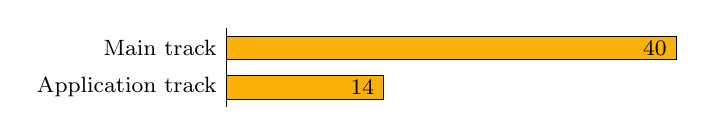
\begin{tikzpicture}
      \draw (0,-.25) -- (0,.75);
      \node [left] at (0,.5) {\footnotesize Main track};
      \node [left] at (0,0) {\footnotesize Application track};
      \draw [fill=yellow!70!red] (0,.35) rectangle (5.714285714,.65);
      \node [left] at (5.714285714,.5) {\footnotesize 40};
      \draw [fill=yellow!70!red] (0,-.15) rectangle (2,.15);
      \node [left] at (2,0) {\footnotesize 14};
    \end{tikzpicture}
  \item Benchmarks:\\
    \smallskip
    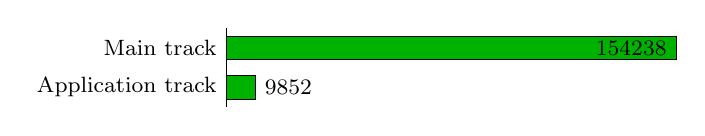
\begin{tikzpicture}
      \draw (0,-.25) -- (0,.75);
      \node [left] at (0,.5) {\footnotesize Main track};
      \node [left] at (0,0) {\footnotesize Application track};
      \draw [fill=green!70!black] (0,.35) rectangle (5.714285714,.65);
      \node [left] at (5.714285714,.5) {\footnotesize 154238};
      \draw [fill=green!70!black] (0,-.15) rectangle (0.365001769,.15);
      \node [right] at (0.365001769,0) {\footnotesize 9852};
    \end{tikzpicture}
  \end{itemize}

  \medskip

  \structure{Record numbers} of solvers, logics, and benchmarks!
\end{frame}

%%%%%%%%%%%%%%%%%%%%%%%%%%%%%%%%%%%%%%%%%%%%%%%%%%%%%%%%%%%%%%%%%%%%%%%%%%%%%%%%

\begin{frame}{Job Pairs}
  \begin{itemize}
  \item \structure{1,028,615} job pairs executed (+ some repeats)
  \item $\sim$ \structure{5 days $\times$ 150 nodes $\times$ 2
    processors/node} of compute time
  \end{itemize}

  \bigskip

  \begin{center}
    \usebeamercolor{structure}
    \begin{tikzpicture}
      \draw [gray] (0,0) -- (7,0);
      \draw [gray] (0,.9) -- (7,.9);
      \draw [gray] (0,1.8) -- (7,1.8);
      \draw [gray] (0,2.7) -- (7,2.7);
      \node [left,gray] at (0,0) {\tiny 0};
      \node [left,gray] at (0,.9) {\tiny 300,000};
      \node [left,gray] at (0,1.8) {\tiny 600,000};
      \node [left,gray] at (0,2.7) {\tiny 900,000};
      \draw [fill=fg] (1,0) rectangle (3,1.019142);
      \draw [fill=fg] (4,0) rectangle (6,3.085845);
      \node [below] at (2,0) {\footnotesize SMT-COMP 2014};
      \node [below] at (5,0) {\footnotesize SMT-COMP 2015};
    \end{tikzpicture}
  \end{center}
  More than \structure{3 times} as many job pairs as in 2014!
\end{frame}

%%%%%%%%%%%%%%%%%%%%%%%%%%%%%%%%%%%%%%%%%%%%%%%%%%%%%%%%%%%%%%%%%%%%%%%%%%%%%%%%

\begin{frame}{StarExec}
  \begin{itemize}
  \item All job pairs executed on StarExec
  \item Over 9,000 job pairs/hour completed
  \end{itemize}

  \medskip
  
  \begin{center}
    {\Large\structure{StarExec worked great}}
  \end{center}

  \medskip
  
  \begin{itemize}
  \item Thanks to Aaron Stump for prompt help when problems or
    questions arose
  \item $\sim$ 20 feature requests and (minor) bug reports submitted
    to the StarExec developers
  \end{itemize}
\end{frame}

%%%%%%%%%%%%%%%%%%%%%%%%%%%%%%%%%%%%%%%%%%%%%%%%%%%%%%%%%%%%%%%%%%%%%%%%%%%%%%%%

\begin{frame}{Machine Specifications}

\end{frame}

%%%%%%%%%%%%%%%%%%%%%%%%%%%%%%%%%%%%%%%%%%%%%%%%%%%%%%%%%%%%%%%%%%%%%%%%%%%%%%%%

\end{document}

%%%%%%%%%%%%%%%%%%%%%%%%%%%%%%%%%%%%%%%%%%%%%%%%%%%%%%%%%%%%%%%%%%%%%%%%%%%%%%%%

% Local Variables:
% ispell-local-dictionary: "american"
% mode: LaTeX
% mode: flyspell
% LocalWords: Tjark
% End:
